\subsection{Specialized Two-Party Bounds}

The previous proofs show that $\TRAV_2$ is maximally complicated in terms of deterministic communication complexity and public randomized communication complexity. A natural follow up question is to ask if we can do better. That is, given some additional constraints, can we solve the problem with reduced communication complexity?

\begin{definition}
Define the $\CTRAV_2$ problem as a $\TRAV_2$ problem where $G_A$ and $G_B$ are guaranteed to be connected subgraphs of $G$.
\end{definition}

\begin{claim}
\label{claim:ctrav}
$\CTRAV_2$ is at least as hard as $\DISJ$. Thus, $D(\CTRAV_2) = \Theta(n)$ and $R(\CTRAV_2) = \Theta(n)$.
\end{claim}

\begin{proof} Let $x,y$ be inputs of Alice and Bob to the $\DISJ$ problem. We construct a graph $G$ as follows: Give ownership of $v$ and all vertices labelled $a_i$ and $i$ if $x_i = 1$, for $i \in [n]$. Similarly for $w$, $G_B$, and $y$. Then if there is a path from $v$ to $w$, this means $\exists i \in [n]$ such that $x_i = y_i = 1$. This means that $S_A \cap S_B \neq \emptyset$. On the other hand, if there is no path from $v$ to $w$, then for all $i \in [n]$, either $x_i = 0$ or $y_i = 0$.

\begin{center}
\begin{figure}[H]
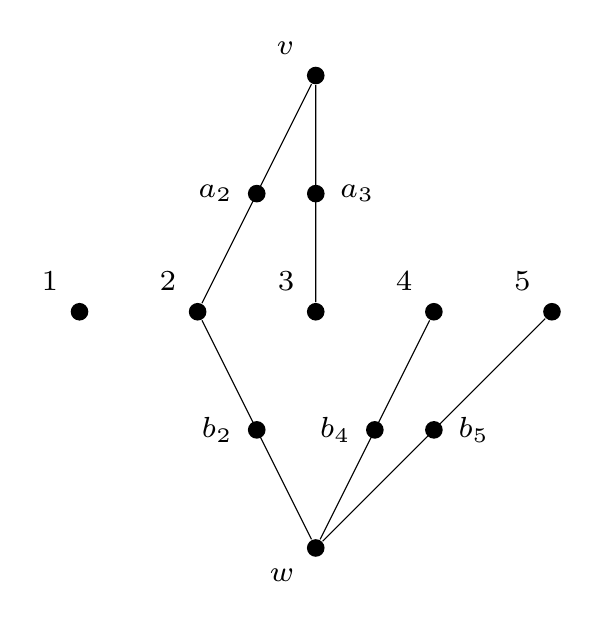
\begin{tikzpicture}[scale=1.5, transform shape]

\node[circle, label=above left:{\scriptsize 1}, fill=black, inner sep=1.5pt] (1) at (1,0) {};
\node[circle, label=above left:{\scriptsize 2}, fill=black, inner sep=1.5pt] (2) at (2,0) {};
\node[circle, label=above left:{\scriptsize 3}, fill=black, inner sep=1.5pt] (3) at (3,0) {};
\node[circle, label=above left:{\scriptsize 4}, fill=black, inner sep=1.5pt] (4) at (4,0) {};
\node[circle, label=above left:{\scriptsize 5}, fill=black, inner sep=1.5pt] (5) at (5,0) {};

\node[circle, label=above left:{\scriptsize $v$}, fill=black, inner sep=1.5pt] (v) at (3,2) {};
\node[circle, label=below left:{\scriptsize $w$}, fill=black, inner sep=1.5pt] (w) at (3,-2) {};

\draw (v) -- (2) node[midway, circle, fill=black, inner sep=1.5pt, label=left:{\scriptsize $a_2$}] {};
\draw (v) -- (3) node[midway, circle, fill=black, inner sep=1.5pt, label=right:{\scriptsize $a_3$}] {};

\draw (w) -- (2) node[midway, circle, fill=black, inner sep=1.5pt, label=left:{\scriptsize $b_2$}] {};
\draw (w) -- (4) node[midway, circle, fill=black, inner sep=1.5pt, label=left:{\scriptsize $b_4$}] {};
\draw (w) -- (5) node[midway, circle, fill=black, inner sep=1.5pt, label=right:{\scriptsize $b_5$}] {};

\end{tikzpicture}
\caption{A $\DISJ$ embedding into $\CTRAV$ with $n = 5$. There is a path from $v$ to $w$ if and only if $\exists i \in [n]$ with $x_i = y_i = 1$.}
\label{fig:ctrav-gadget}
\end{figure}
\end{center}

We note that $|V(G_A)| = |V(G_B)| = |x| = |y| = \Theta(n)$. Furthermore, $G_A$ and $G_B$ are connected subgraphs of $G$. This completes the reduction.
\end{proof}

% 
\begin{figure} [H]
\begin{center}
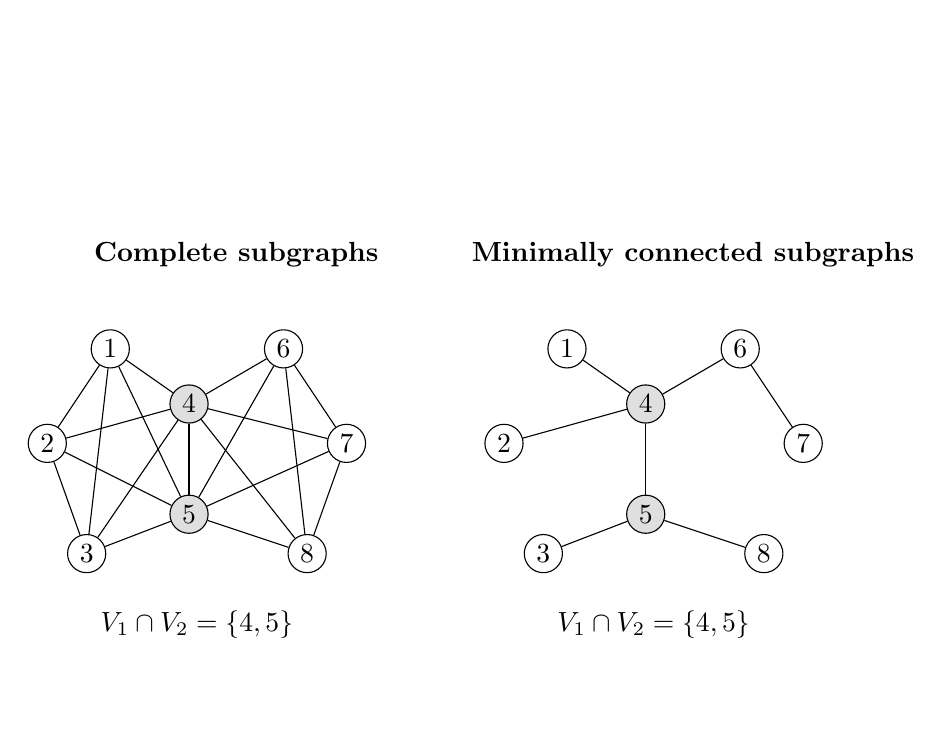
\begin{tikzpicture}[
  scale=1.0,
  every node/.style={circle, draw, fill=white, inner sep=2pt},
  shared/.style={fill=gray!25},
  lab/.style={draw=none, fill=none, font=\bfseries}
]

% =======================
% Panel A: Complete graphs
% =======================
\node[lab] (titleA) at (0,2.6) {Complete subgraphs};

% Nodes (left panel)
\node (A1) at (-1.6, 1.4) {1};
\node (A2) at (-2.4, 0.2) {2};
\node (A3) at (-1.9,-1.2) {3};

\node[shared] (A4) at (-0.6, 0.7) {4};
\node[shared] (A5) at (-0.6,-0.7) {5};

\node (A6) at ( 0.6, 1.4) {6};
\node (A7) at ( 1.4, 0.2) {7};
\node (A8) at ( 0.9,-1.2) {8};

% K5 on {1,2,3,4,5}
\foreach \u/\v in {A1/A2,A1/A3,A1/A4,A1/A5,A2/A3,A2/A4,A2/A5,A3/A4,A3/A5,A4/A5}{
  \draw (\u)--(\v);
}

% K5 on {4,5,6,7,8}
\foreach \u/\v in {A4/A5,A4/A6,A4/A7,A4/A8,A5/A6,A5/A7,A5/A8,A6/A7,A6/A8,A7/A8}{
  \draw (\u)--(\v);
}

\node[lab] at (-0.5,-2.1) {$V_1\cap V_2=\{4,5\}$};

% =======================
% Panel B: Minimal (trees)
% =======================
\node[lab] (titleB) at (5.8,2.6) {Minimally connected subgraphs};

% Nodes (right panel) — same geometry shifted right
\node (B1) at (4.2, 1.4) {1};
\node (B2) at (3.4, 0.2) {2};
\node (B3) at (3.9,-1.2) {3};

\node[shared] (B4) at (5.2, 0.7) {4};
\node[shared] (B5) at (5.2,-0.7) {5};

\node (B6) at (6.4, 1.4) {6};
\node (B7) at (7.2, 0.2) {7};
\node (B8) at (6.7,-1.2) {8};

% Tree on {1,2,3,4,5} (4 edges)
\draw (B4)--(B1);
\draw (B4)--(B2);
\draw (B5)--(B3);
\draw (B4)--(B5);

% Tree on {4,5,6,7,8} (4 edges)
\draw (B4)--(B6);
\draw (B6)--(B7);
\draw (B5)--(B8);
\draw (B4)--(B5);

\node[lab] at (5.3,-2.1) {$V_1\cap V_2=\{4,5\}$};

% =======================
% Caption / statement
% =======================
\end{tikzpicture}
\caption{Same vertex sets $V_1=\{1,2,3,4,5\},V_2=\{4,5,6,7,8\}$ in both panels.
Changing edges (complete vs tree) does not change $V_1\cap V_2$.}
\end{center}

\end{figure}


Informally, this tells us that even when $G_A$ and $G_B$ are connected subgraphs, we do not immediately get better bounds and the problem does not become significantly easier. We now consider a sparser case:

\begin{definition}
Define $\STRAV_2$ as a $\TRAV_2$ problem where $E(G) = O(n)$, $E(G_A) = O(n)$, and $E(G_B) = O(n)$. In other words, the graph $G$ is sparse and $G_A$, $G_B$ are sparse too.
\end{definition}

\begin{claim}
\label{claim:strav}
$\STRAV_2$ is at least as hard as $\DISJ$. Thus, $D(\STRAV_2) = \Theta(n)$ and $R(\STRAV_2) = \Theta(n)$.
\end{claim}

\begin{proof}
We reuse the reduction from $\DISJ$ to $\TRAV_2$ in Claim \ref{claim:disjoint-trav-bound}. In that construction, $G$ is a chain of $n$ disjointness gadgets, so $|E(G)| = \Theta(n)$. Moreover, each player's subgraph consists of the gadget boundary vertices and one branch choice per gadget, which also gives $|E(G_A)| = \Theta(n)$ and $|E(G_B)| = \Theta(n)$.

Hence every instance produced by that reduction already satisfies the sparsity constraints in the definition of $\STRAV_2$. The reduction still preserves correctness: $\DISJ(x,y)=1$ iff there is a $v$ to $w$ path in $G_A \cup G_B$. Therefore $\STRAV_2$ is at least as hard as $\DISJ$.
\end{proof}

Informally, this tells us that weak edge sparsity of $G$, $G_A$, and $G_B$ does not add nor remove significant communication cost. Combined with Claim \ref{claim:ctrav}, this may imply that the local structure of $G$, $G_A$, and $G_B$, namely, how sparse or connected the edges corresponding to the owned vertices are, do not have a significant impact on the deterministic and pubic randomized communication complexity of the $\TRAV_2$ problem.
